\documentclass[tikz,border=5pt]{standalone}
\usepackage{amsmath}
\usepackage{amssymb}
\usepackage{xcolor}
\usepackage{tikz}
\usetikzlibrary{
    arrows.meta,
    positioning,
    shapes.geometric,
    fit,
    backgrounds,
    calc
}
\begin{document}
\pagecolor{white}

% show background rectangle, background rectangle/.style={fill=white},
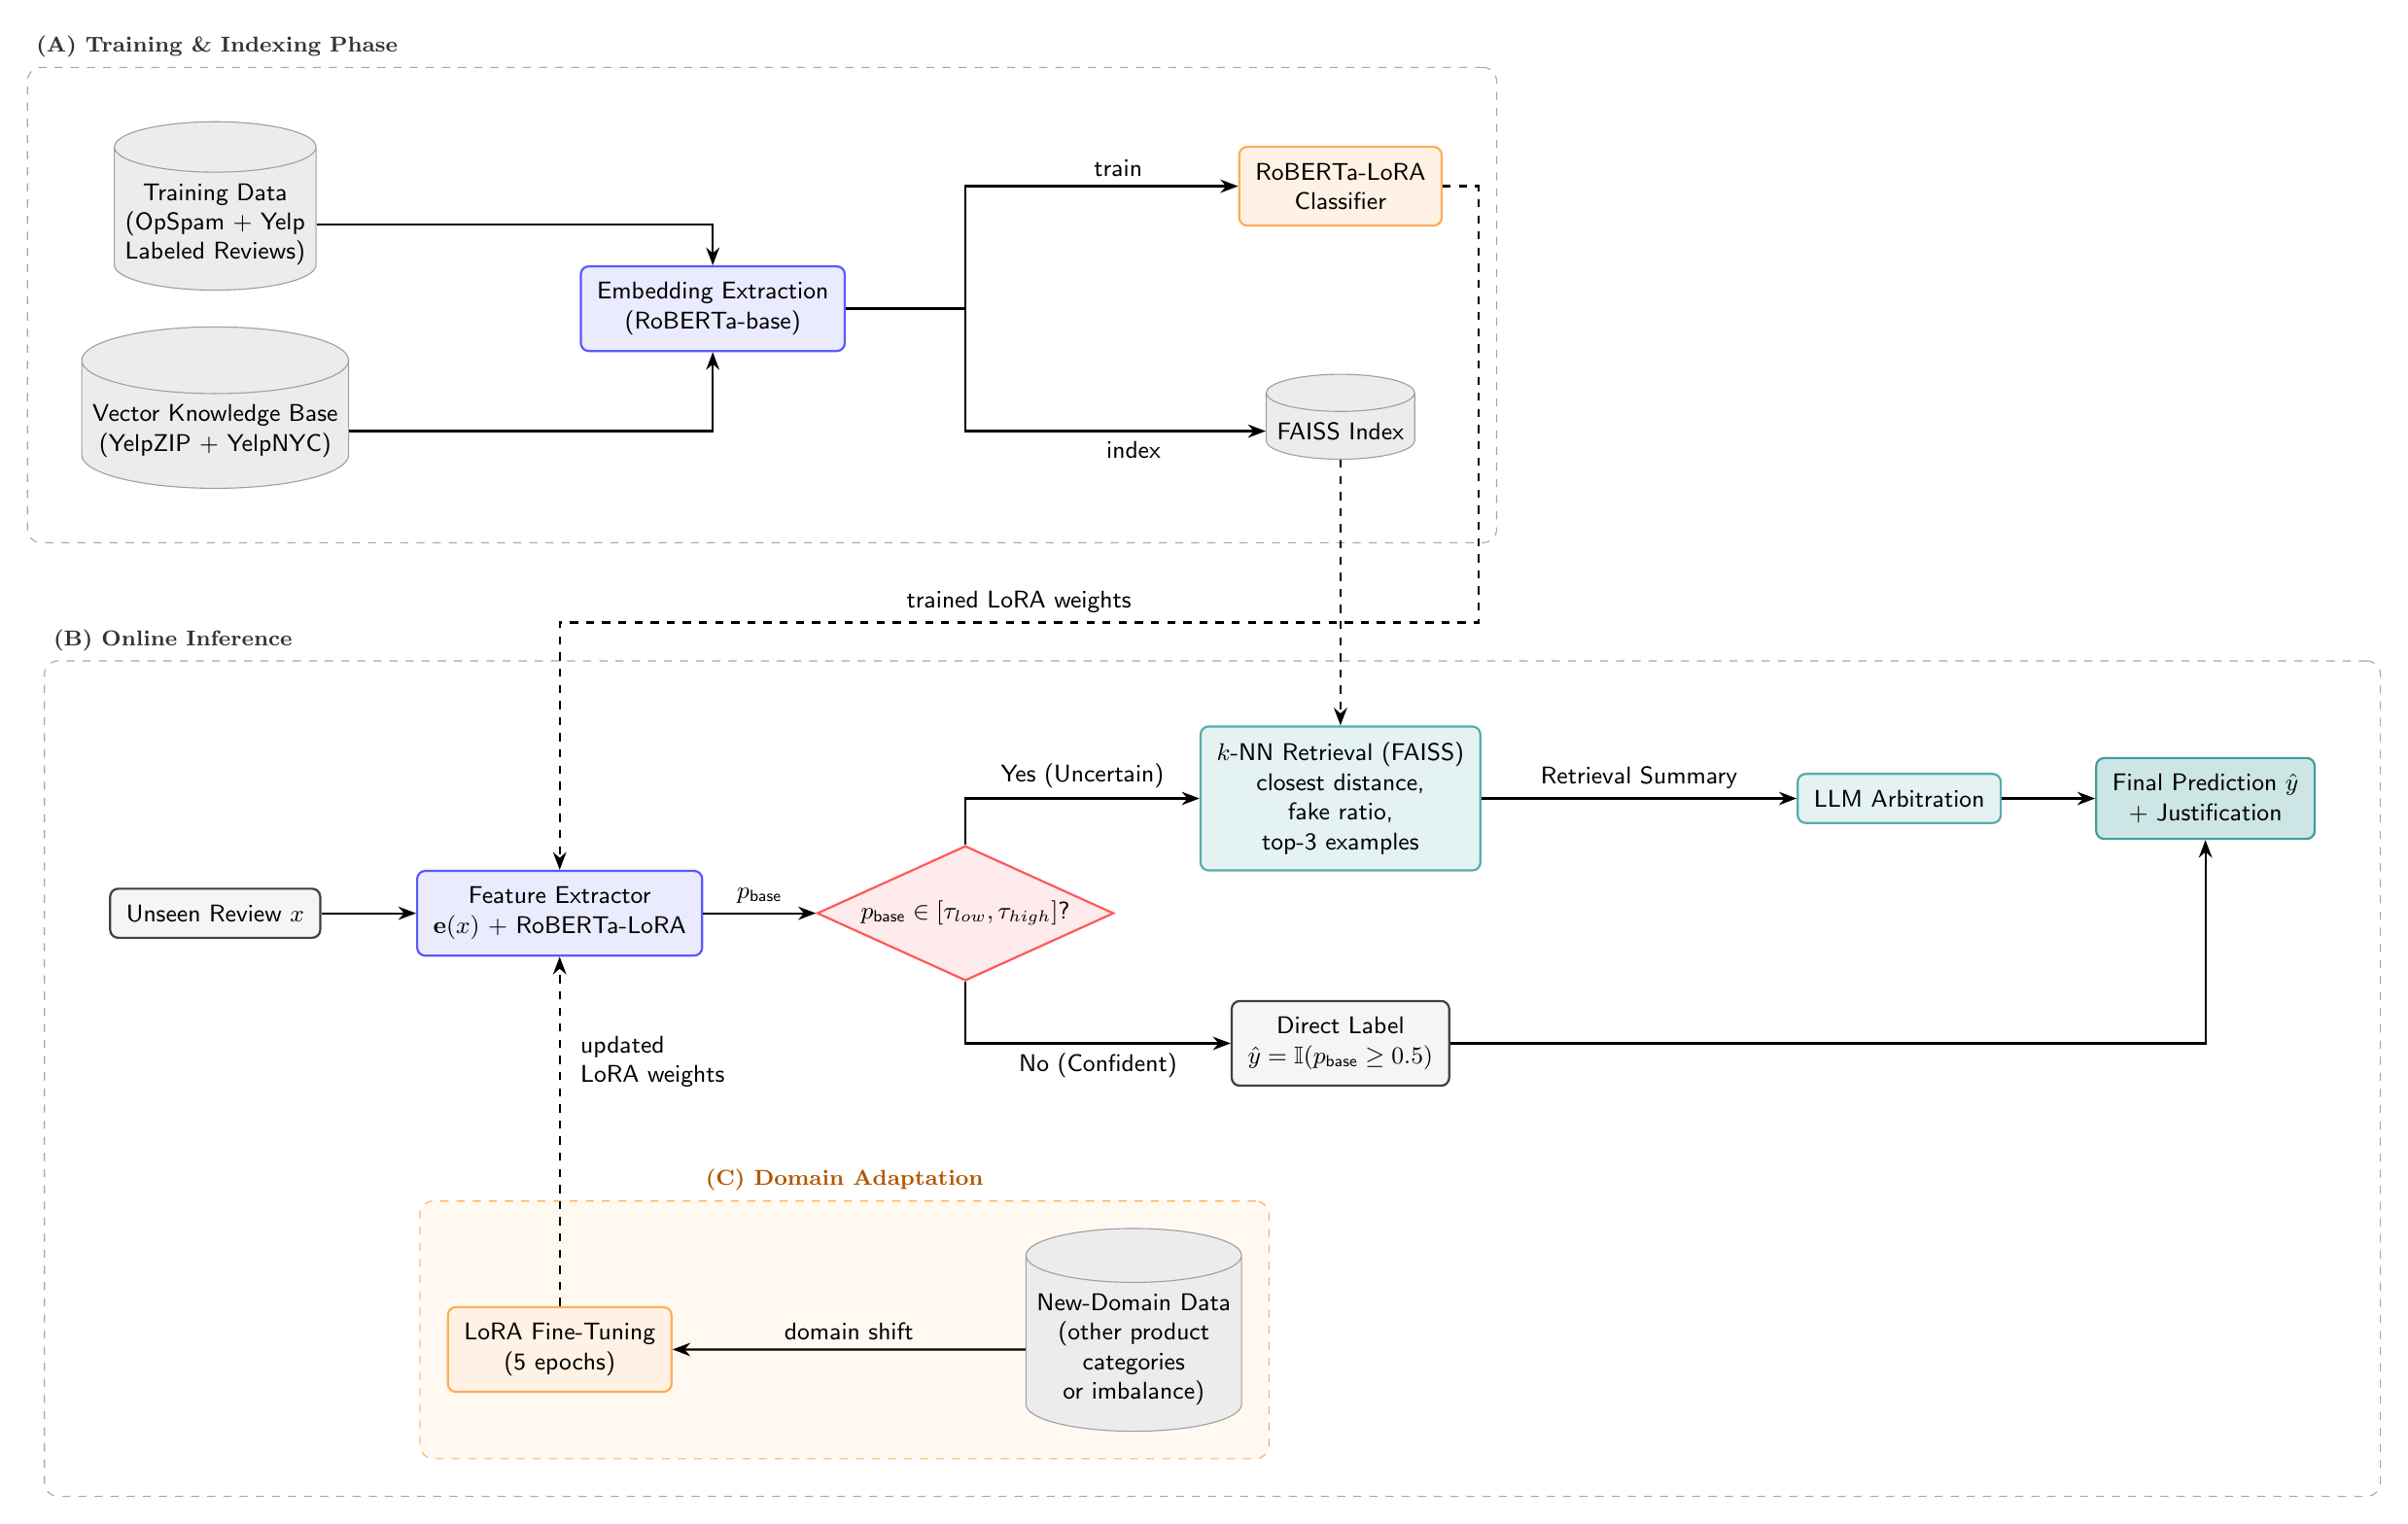
\begin{tikzpicture}[
    >=Stealth,
    font=\small\sffamily,
    box/.style={draw=black!75, fill=gray!8, rounded corners=3pt, align=center, inner sep=6pt, line width=0.8pt},
    proc/.style={box, fill=blue!8, draw=blue!65},
    clf/.style={box, fill=orange!10, draw=orange!65},
    rag/.style={box, fill=teal!10, draw=teal!65},
    decision/.style={diamond, draw=red!65, fill=red!8, aspect=2.2, inner sep=2pt, line width=0.8pt, align=center},
    data/.style={cylinder, draw=gray!75, fill=gray!15, shape border rotate=90, aspect=0.25, inner sep=4pt, align=center},
    subframe/.style={draw=black!35, dashed, rounded corners=5pt, inner sep=20pt, fill=none},
    framelabel/.style={anchor=south west, font=\footnotesize\bfseries, text=black!80}
]


% ================= (A) Offline Phase =================
\node[data] (train) at (0,-0.5)
    {Training Data\\(OpSpam + Yelp\\Labeled Reviews)};
\node[data] (vector) at (0,-3.2)
    {Vector Knowledge Base \\(YelpZIP + YelpNYC)};

\node[proc] (embed) at (6.5,-1.6)
    {Embedding Extraction\\(RoBERTa-base)};

\node[clf]  (classifier) at (14.7,0)
    {RoBERTa-LoRA\\Classifier};
\node[data] (faiss) at (14.7,-3.2)
    {FAISS Index};

\coordinate (split) at (9.8,-1.6);

\draw[->, thick] (train.east) -| (embed.north);
\draw[->, thick] (vector.east) -| (embed.south);
\draw[thick] (embed.east) -- (split);
\draw[->, thick] (split) |- node[above, pos=0.78] {train} (classifier.west);
\draw[->, thick] (split) |- node[below, pos=0.78] {index} (faiss.west);

% ================= (B) Online Inference Phase =================
\node[box] (input) at (0,-9.5) {Unseen Review $x$};
\node[proc] (query_embed) at (4.5,-9.5)
    {Feature Extractor\\$\mathbf{e}(x)$ + RoBERTa-LoRA};
\node[decision] (check) at (9.8,-9.5) {$p_{\text{base}}\in [\tau_{low}, \tau_{high}]$?};

\node[rag] (retrieve) at (14.7,-8)
    {$k$-NN Retrieval (FAISS)\\closest distance,\\fake ratio,\\ top-3 examples};
\node[rag] (llm) at (22,-8) {LLM Arbitration};
\node[box, fill=teal!20, draw=teal!75] (output) at (26,-8)
    {Final Prediction $\hat{y}$\\+ Justification};

\node[box] (direct) at (14.7,-11.2) {Direct Label\\$\hat{y} = \mathbb{I}(p_{\text{base}} \ge 0.5)$};

\draw[->, thick] (input) -- (query_embed);
\draw[->, thick] (query_embed) -- node[above] {$p_{\text{base}}$} (check);
\draw[->, thick] (check.north) |- node[pos=0.75, above] {Yes (Uncertain)} (retrieve.west);
\draw[->, thick] (check.south) |- node[pos=0.75, below] {No (Confident)} (direct.west);
\draw[->, thick] (retrieve) -- node[above] {Retrieval Summary} (llm);
\draw[->, thick] (llm) -- (output);
\draw[->, thick] (direct.east) -| (output.south);

% Connections: FAISS index -> retrieval / Classifier -> e(x) + RoBERTa-LoRA
\draw[->, thick, dashed] (faiss.south) -- (retrieve.north);
\coordinate (w1) at (16.5,0);
\coordinate (w2) at (16.5,-5.7);
\coordinate (w3) at (4.5,-5.7);
\draw[->, thick, dashed] (classifier.east) -- (w1) -- (w2)
    -- node[above] {trained LoRA weights} (w3)
    -- (query_embed.north);
% ================= (C) Domain Adaptation =================
\node[data] (newdom) at (12,-15.2)
    {New-Domain Data\\(other product\\categories\\or imbalance)};
\node[clf] (adapt) at (4.5,-15.2)
    {LoRA Fine-Tuning\\(5 epochs)};

\draw[->, thick] (newdom) -- node[above] {domain shift} (adapt);
\draw[->, thick, dashed] (adapt.north) -- node[pos=0.7, right=4pt, align=left] {updated\\LoRA weights} (query_embed.south);
% ================= Frames =================
\begin{scope}[on background layer]
    %\node[fit=(vector)(train)(embed)(classifier)(faiss)(input)(query_embed)(check)(direct)(retrieve)(llm)(output)(newdom)(adapt),
    %      fill=white,
    %      draw=none,
    %      inner sep=15pt] (mainbg) {};
    \node[subframe, fit=(vector)(train)(embed)(classifier)(faiss),
          label={[framelabel]north west:(A) Training \& Indexing Phase}] (frameA) {};

    \node[subframe, inner sep=24pt,
          fit=(input)(query_embed)(check)(direct)(retrieve)(llm)(output)(newdom)(adapt),
          label={[framelabel]north west:(B) Online Inference}] (frameB) {};

    \node[subframe, draw=orange!65, fill=orange!5, inner sep=10pt, fit=(newdom)(adapt),
          label={[framelabel, anchor=south, text=orange!70!black]north:(C) Domain Adaptation}] (frameC) {};
\end{scope}

\end{tikzpicture}

\end{document}
